% Two overlapping pieces of X with A (orange) in their overlap around a point Z.
% Source: book/tex/homology/excision.tex (§ The excision theorem).
\documentclass[border=2mm]{standalone}
\usepackage{tikz}
\begin{document}
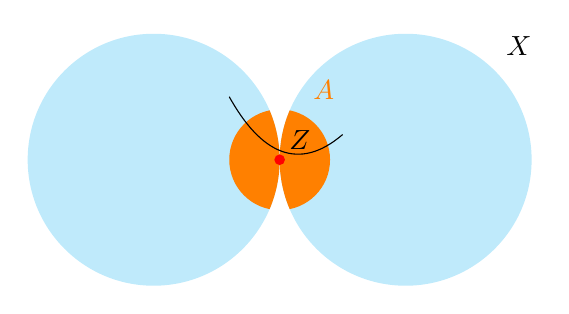
\begin{tikzpicture}[scale=1.6]
  \fill[cyan!25] (0,0) circle (1);
  \fill[cyan!25] (2,0) circle (1);
  \begin{scope} \clip (0,0) circle (1); \fill[orange] (1,0) circle (0.4); \end{scope}
  \begin{scope} \clip (2,0) circle (1); \fill[orange] (1,0) circle (0.4); \end{scope}
  \node at (2.9,0.9) {$X$};
  \node[orange] at (1.35,0.55) {$A$};
  \fill[red] (1,0) circle (1.2pt); \node[above right] at (1,0) {$Z$};
  \draw (0.6,0.5) .. controls (0.85,0.05) and (1.15,-0.1) .. (1.5,0.2);
\end{tikzpicture}
\end{document}
